\documentclass{beamer}

\usepackage{graphicx}
\graphicspath{/}

\title{Proyecto Final: Resumen}
\author{Rolando Rivas 594276, Diego Estrada 627760, Francisco Javier Camara 636930}
\date{5 de Diciembre del 2023}

\begin{document}

\frame{\titlepage}

\begin{frame}{Introducción: La luz}
    \begin{itemize}
        \item La luz es una forma de energia en forma de ondas electromagnéticas y particulas
        \item Es una onda porque tiene caracteristicas propias de las ondas: longitud de onda, amplitud, frecuencia. etc.
        \item Es tambien particula porque puede interactuar con la materia, transmitiendo energia, reflejando, absorbiendo, etc.
        \item Las plantas hacen uso de esta propiedad de absorción de la luz para fabricar energía.
    \end{itemize}
\end{frame}

\begin{frame}{Reflexion y Absorción}
    \begin{itemize}
        \item La luz al interactuar con la materia puede reflejarse o absorberse.
        \item Al ser una onda la luz, ciertas longitudes de onda pueden ser absorbidas o reflejadas. Por eso diferentes materiales tienen colores diferentes.
        \item Las ondas reflejadas son visibles para el ojo y las absorbidas no
        \item Se es posible conocer qué materiales posee una planta dependiendo de las longitudes de onda que refleje y absorba.
    \end{itemize}
\end{frame}

\begin{frame}{Espectrómetro y sus Componentes}
    \begin{itemize}
        \item Un espectrómetro identifica las longitudes de onda absorbidas y reflejadas mandando una emisión de ondas electromagneticas.
        \item   Es capaz de generar las longitudes de onda de Ultravioleta, Infrarrojo y Luz Visible. 
        \item Componentes principales: entrada de luz, elemento dispersivo y detector.
    \end{itemize}
\end{frame}

\begin{frame}{Materiales y Métodos}
    \begin{itemize}
        \item Clorofito Comosum, Mexican BlueBell (Tallo y Hoja)
        \item Jeringa,  Espectrometro, Agua Destilada, Ethanol, Mortero
        \item Metodología seguida para la preparación de las muestras y el análisis.
    \end{itemize}
\end{frame}

\begin{frame}{Resultados Clorofito Comosum}
    \begin{itemize}
        \item Resultados obtenidos para las plantas evaluadas.
    \end{itemize}
    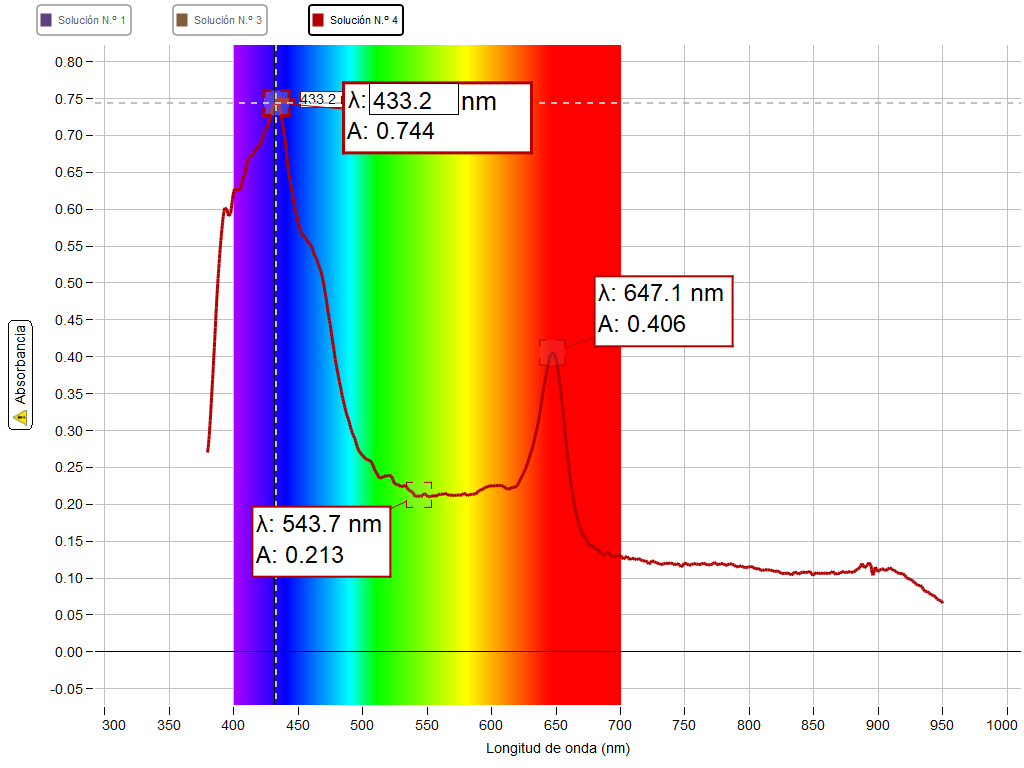
\includegraphics[scale=0.3]{clorofitoComosumCoordenadas.png}
\end{frame}

\begin{frame}{Resultados Mexican Bluebell Hoja}
    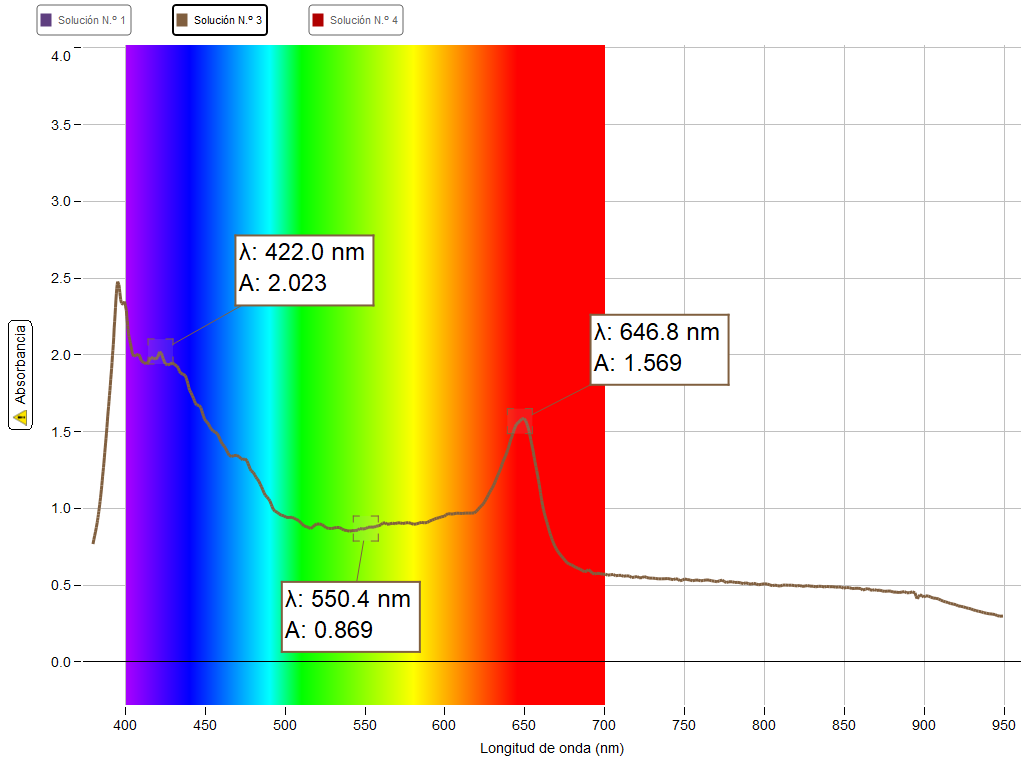
\includegraphics[scale=0.3]{MexicanBluebelHOJAcoorenadas.png}
\end{frame}

\begin{frame}{Resultados Mexican Bluebell Tallo}
    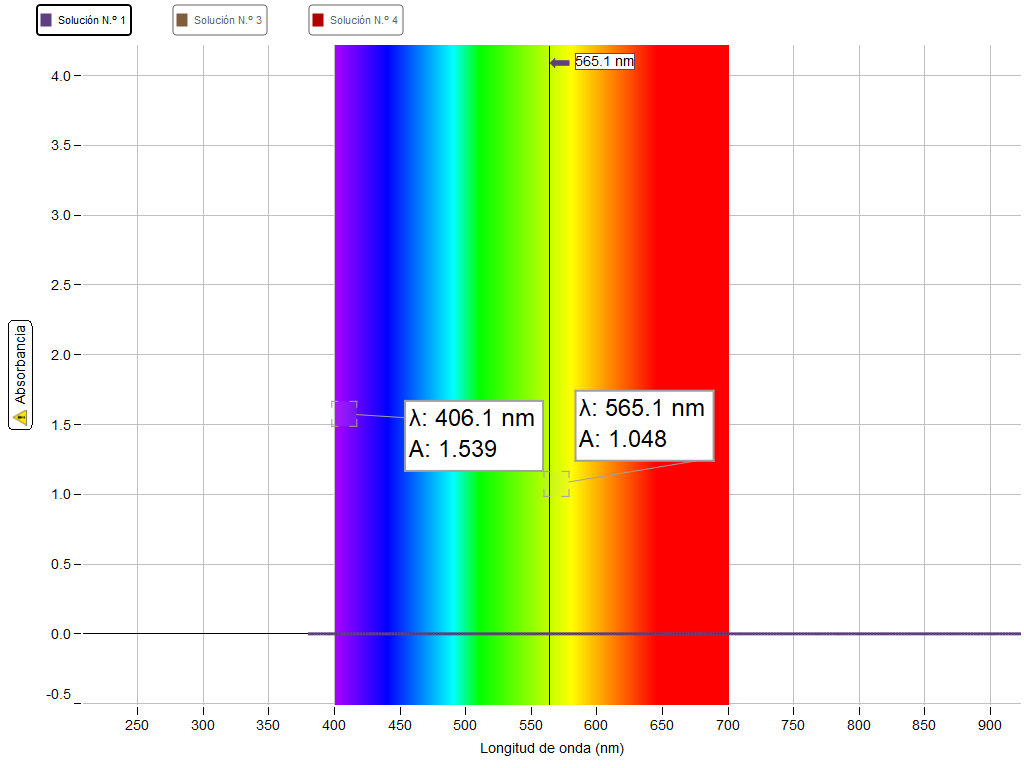
\includegraphics[scale=0.3]{mexicanBluebellCoordenadas.png}
\end{frame}

\begin{frame}{Discusiones}
    \begin{itemize}
        \item Resumen de las observaciones clave.
        \item Implicaciones de los hallazgos.
    \end{itemize}
\end{frame}

\begin{frame}{Referencias}
   \small [1]...Artedinamico. (2022). LA LUZ. Equipos Y Laboratorio de Colombia. https://www.equiposylaboratorio.com/portal/inicio
[2]‌…Clase 3. (n.d.). https://sistemas.fciencias.unam.mx/~fam/Cursos/Cuantica/Clases/clase3.pdf
[3]...Vista de Descargas eléctricas y sus aplicaciones. (2023). Ufps.edu.co. https://revistas.ufps.edu.co/index.php/ecomatematico/article/view/447/1591#:~:text=Si%20le%20entregamos%20energ%C3%ADa%20a,de%20electrones%20capaces%20de%20ionizar.
[4]‌…Admin. (2019, August 5). Emission Spectrum - Definition, Types, Examples | Hydrogen Transitions. BYJUS; BYJU’S. https://byjus.com/physics/emission-spectrum/
‌[5]...Visible Light - NASA Science. (2016, August 10). Nasa.gov. https://science.nasa.gov/ems/09_visiblelight/
[6]...Spectroscopy 101 – How Absorption and Emission Spectra Work. (2021). Webb; Q Starter Kit. https://webbtelescope.org/contents/articles/spectroscopy-101--how-absorption-and-emission-spectra-work#:~:text=Different%20elements%20have%20different%20spectra,electrons%20move%20between%20energy%20levels.
‌[7]...Fernandes, A. (2016). Espectro de absorción - Knoow. Knoow.net. https://knoow.net/es/ciencias-tierra-vida/biologia-es/espectro-de-absorcion/
‌[8]...¿Qué es un espectrómetro? Explicación del espectrómetro UV, VIS e IR. (2020, April 29). Wavelength Opto-Electronic. https://wavelength-oe.com/es/articles/what-is-a-spectrometer/
\end{frame}

\end{document}
